\chapter{Hardware Testings}
The designed microcontroller will be implemented on Arrow DECA FPGA board.
This board has Altera MAX 10 10M50DAF484C6G device with 50K programmable logic elements and other useful elements for future developements.
Three tests will be conducted using this board: Output testings, Input testings and UART Transmission testings along with the sample programs and breif explanations.

\section{Sample Output Program}
This program counts from 0 to 6 and loops back to 0.
The program outputs the counter value as a binary on the lower 3 pin of general I/O port.
The test program is the following.
\begin{table}[!h]
    \centering
    \caption{Sample Output Program}
    \label{program:sample_output}
    \begin{tabular}{|c|l|l|}
        \hline
        \textbf{Line} & \textbf{Instruction} & \textbf{Description}       \\ \hline
        1             & addi x1 x0 0         & set general io as output   \\ \hline
        2             & addi x4 x0 6         & set threshold limit        \\ \hline
        3             & sd x1 x0 1           &                            \\ \hline
        4             & addi x3 x0 0         & initialize counter         \\ \hline
        5             & L1: addi x3 x3 1     & add 1 to counter           \\ \hline
        6             & sd x3 x0 2           & write to general io        \\ \hline
        7             & bne x4 x3 L1         & loop back if not threshold \\ \hline
        8             & addi x3 x0 0         & reset and loop             \\ \hline
        9             & sd x3 x0 2           &                            \\ \hline
        10            & beq x0 x0 L1         &                            \\ \hline
    \end{tabular}

\end{table}

As can be seen below, the counting is working and the outputs are working as well.
\begin{table}
    \center
    \begin{tabular}{cc}
        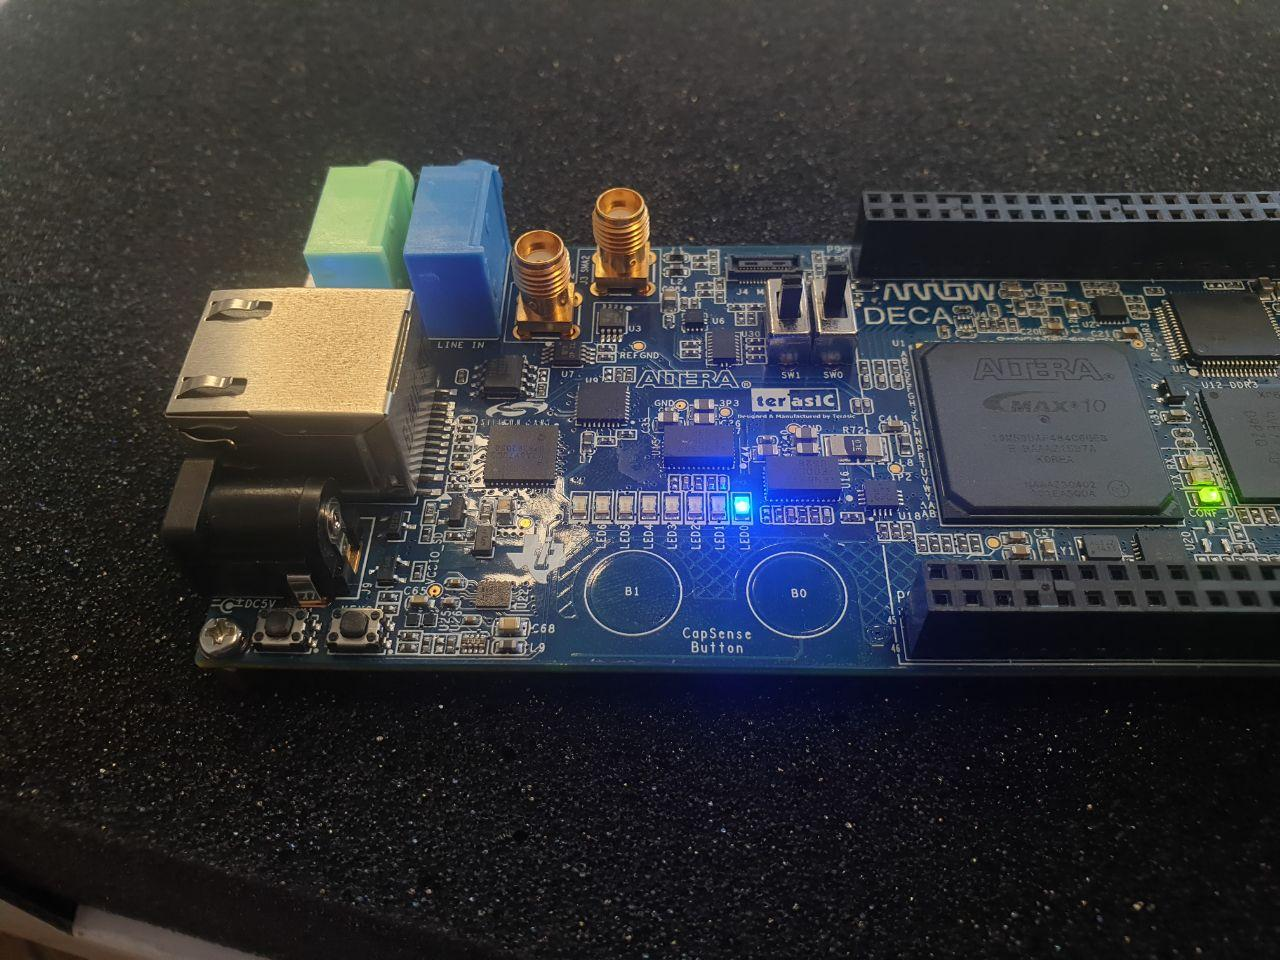
\includegraphics[scale=0.2]{graphics/hardware_output_1} & 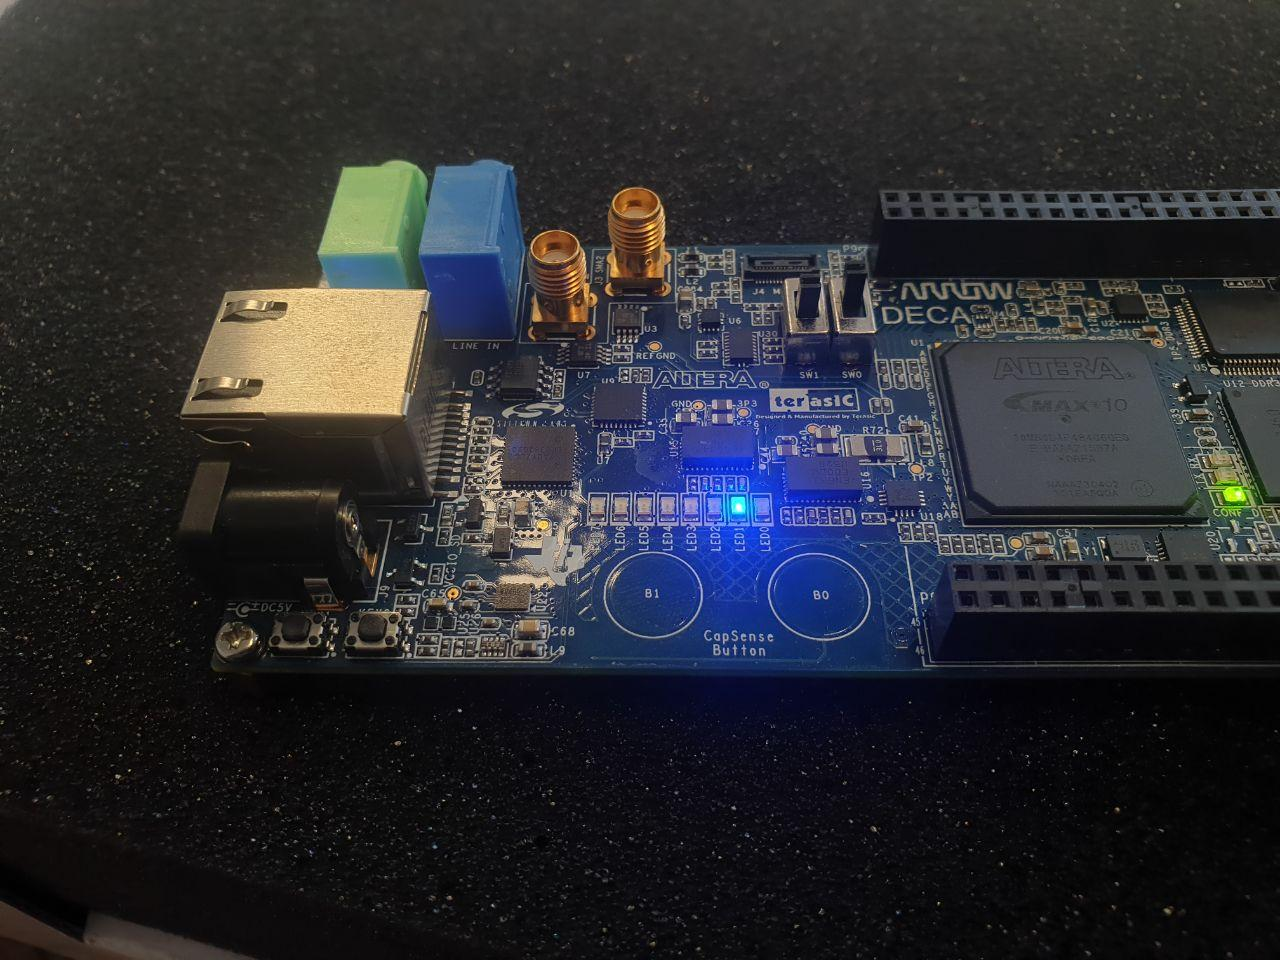
\includegraphics[scale=0.2]{graphics/hardware_output_2} \\
        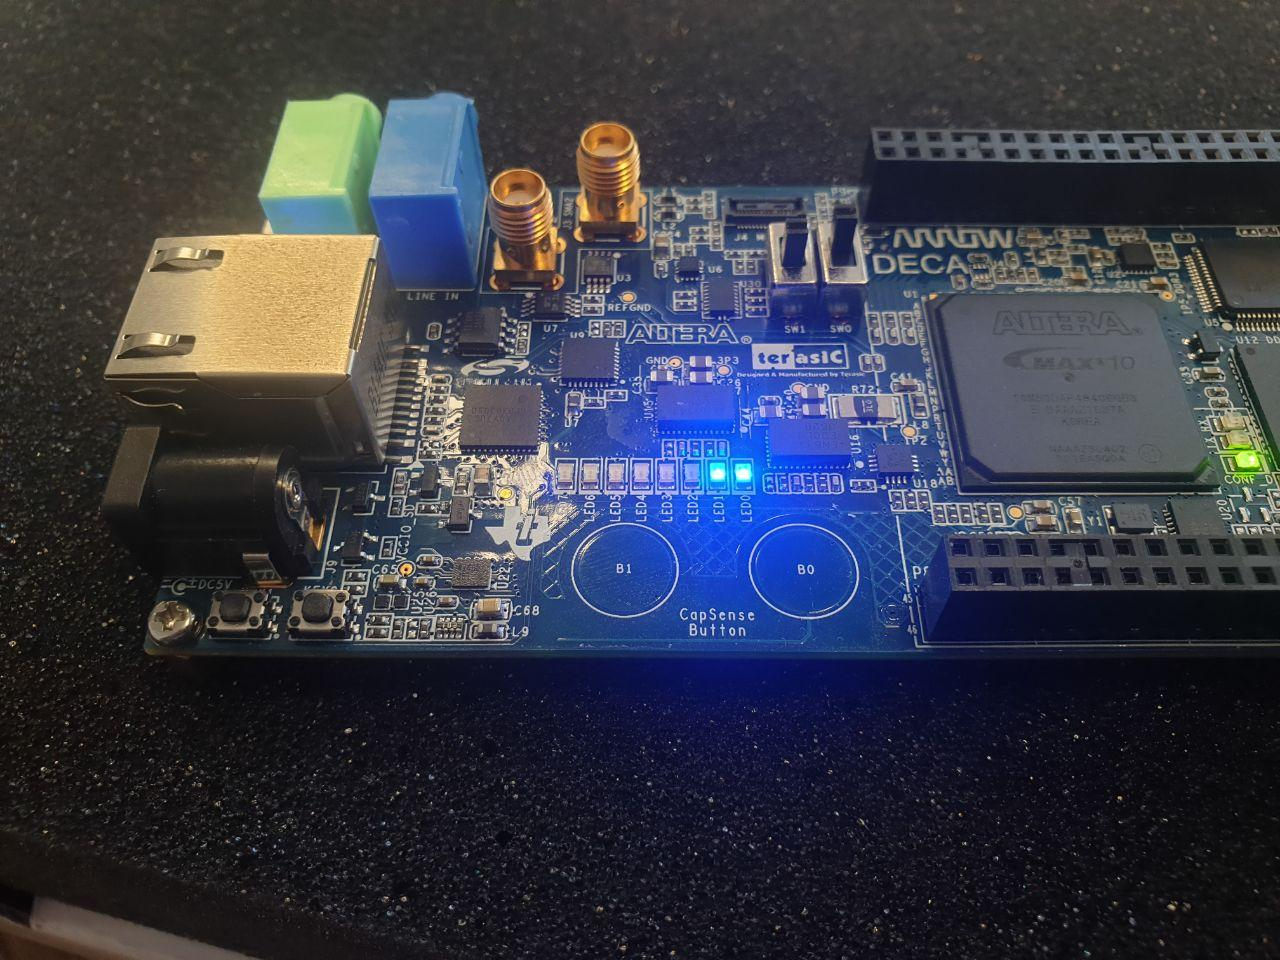
\includegraphics[scale=0.2]{graphics/hardware_output_3} & 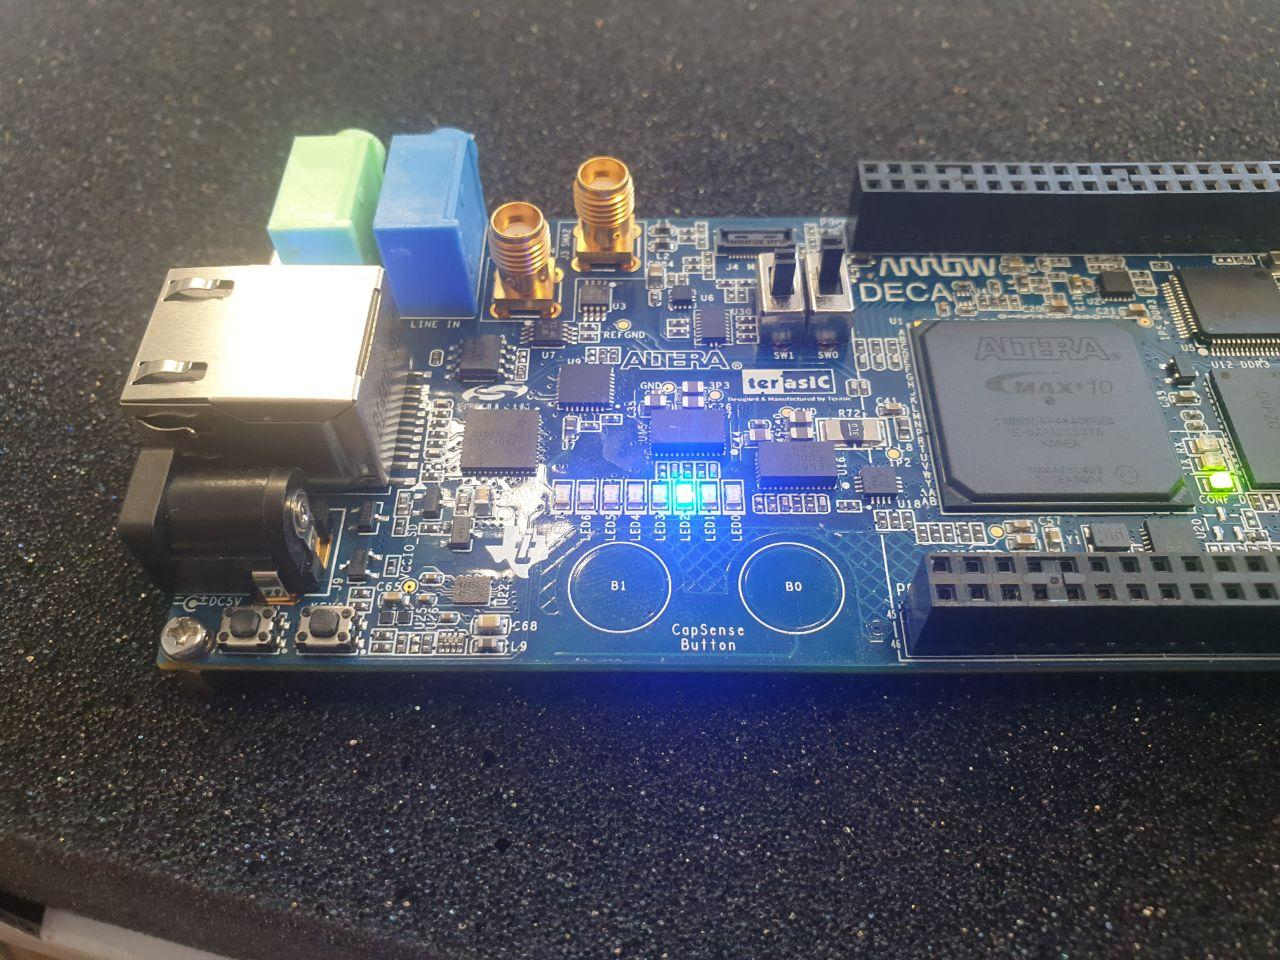
\includegraphics[scale=0.2]{graphics/hardware_output_4} \\
    \end{tabular}
    \caption{Output counting from 1 to 4}
    \label{graphic:output_counting}
\end{table}

\section{Sample Input Program}
This program test the input capabilities of the microcontroller.
It reads the input from the switch and put the value to the output.
The button is configure with pull down configuration, meaning without pressing the button, the input is ground, which is Low.
Upon pressing the button, the input will be 3.3V, which is High.
The output LED is drive accordingly, when input is High, LED is on. When input is Low, LED is off.

\begin{table}[!h]
    \centering
    \caption{Sample Input/Output Program}
    \label{program:sample_io}
    \begin{tabular}{|c|l|l|}
        \hline
        \textbf{Line} & \multicolumn{1}{c|}{\textbf{Instruction}} & \multicolumn{1}{c|}{\textbf{Description}} \\ \hline
        1             & addi x1 x0 16                             & set pin 5 as input                        \\ \hline
        2             & sd x1 x0 1                                &                                           \\ \hline
        3             & L1: ld x3 x0 3                            & read the pin and store into x3            \\ \hline
        4             & and x4 x3 x1                              & Isolate only the input value of pin 5     \\ \hline
        5             & beq x4 x1 L2                              & check if it is 1                          \\ \hline
        6             & addi x5 x0 0                              & set output low if not 1                   \\ \hline
        7             & sd x5 x0 2                                &                                           \\ \hline
        8             & beq x0 x0 L1                              &                                           \\ \hline
        9             & L2: addi x5 x0 1                          & set output high if 1                      \\ \hline
        10            & sd x5 x0 2                                &                                           \\ \hline
        11            & beq x0 x0 L1                              & repeat                                    \\ \hline
    \end{tabular}
\end{table}

As can be observed in Figure \ref{graphic:input_on_off}, the LED is on when the button is pressed and is off when the button is released.\
\begin{table}
    \centering
    \begin{tabular}{cc}
        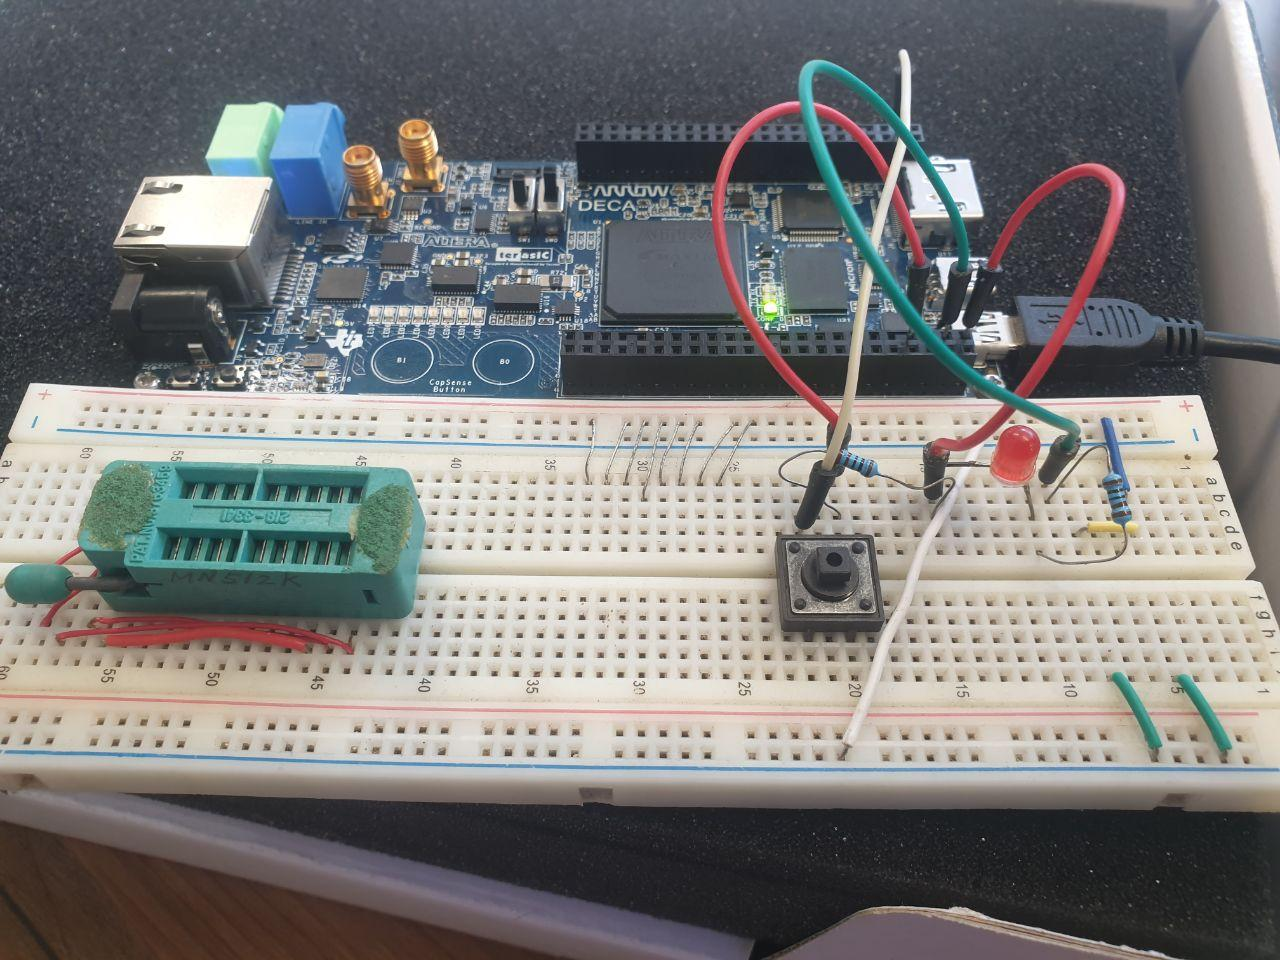
\includegraphics[scale=0.2]{graphics/hardware_input_off} & 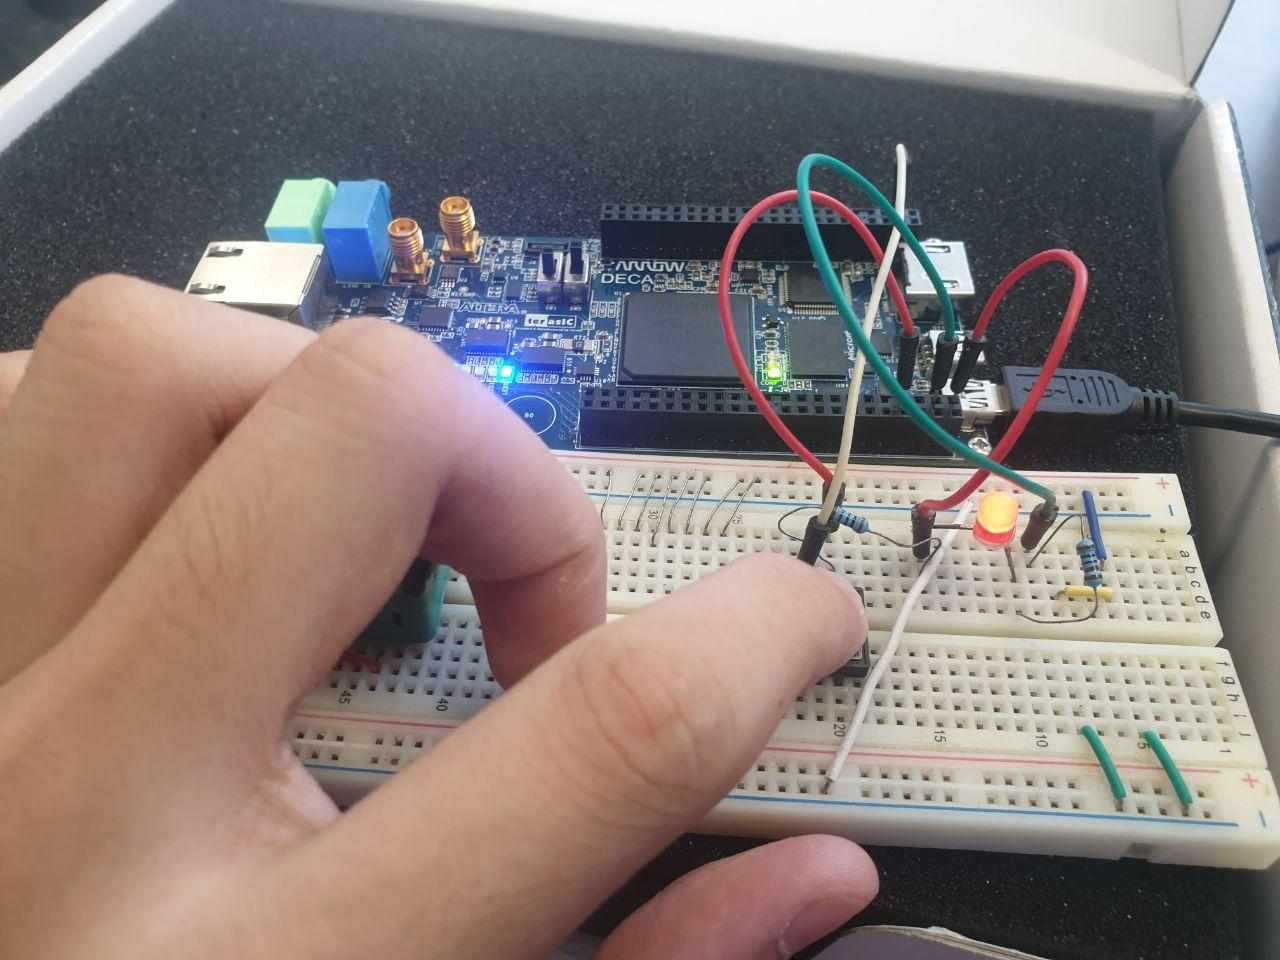
\includegraphics[scale=0.2]{graphics/hardware_input_on}
    \end{tabular}
    \caption{LED turning on button press}
    \label{graphic:input_on_off}
\end{table}

\newpage
\section{Sample UART Transmission Program}
This program tests the transmission of data from UART1 on special I/O.
The program first load the data of 682(1010101010) into the UART1 data write register in Data Memory.
When start signal in UART1 Control register is set, the hardware should start transmitting 4 packet of data, each carrying 1 byte of data.
After that, the TX line should stay in idle state.

\begin{table}[!h]
    \centering
    \caption{Sample UART1 Transmission Program}
    \label{program:sample_uart}
    \begin{tabular}{|c|l|l|}
        \hline
        \textbf{Line} & \multicolumn{1}{c|}{\textbf{Instruction}} & \multicolumn{1}{c|}{\textbf{Description}}    \\ \hline
        1             & addi x1 x0 0                              & clear the control of UART1                   \\ \hline
        2             & sd x1 x0 4                                &                                              \\ \hline
        3             & addi x1 x0 682                            & set the 682 as data to be transmitted        \\ \hline
        4             & sd x1 x0 11                               &                                              \\ \hline
        5             & addi x1 x0 1                              & begin transmitting                           \\ \hline
        6             & sd x1 x0 4                                &                                              \\ \hline
        7             & addi x1 x0 0                              & clear transmitting to only transmit one data \\ \hline
        8             & sd x1 x0 4                                &                                              \\ \hline
        9             & L1:                                       & set output high if 1                         \\ \hline
        10            & beq x0 x0 L1                              & loop                                         \\ \hline
    \end{tabular}
\end{table}

As can be seen in Figure \ref{graphic:hardware_uart}, the data is transmitted and it captured by the oscilloscope.
All four packets of data can be observed as well.

\insertGraphic{hardware_uart}{0.5}{0}{UART1 Transmitting Data}{graphic:hardware_uart}